\scanpage{36}\mspage{35}

On pose
\[
\begin{aligned}
(\deleted{X}A',\sigma')\leq(\deleted{X}A,\sigma)&\overset{\mathrm{dfn}}{\Longleftrightarrow}
(\deleted{X}A',\sigma')\ \text{sous-simplexe \inserted{de $(A,\sigma)$} (face)}\\
(\deleted{X}A',\sigma')\ll(\deleted{X}A,\sigma)&\overset{\mathrm{dfn}}{\Longleftrightarrow}
\overset{\text{\inserted{de $(\deleted{X}A,\sigma)$}}}{\Phi_{\sigma'}\ll\Phi_{\sigma\deleted{\unsure{\prime}}}}\\
(\deleted{X}A,\sigma)\mathrel{\tikz[baseline=-.55ex,x=.85em,y=.70em]{\draw[line cap=round,line join=round] (0,1) .. controls (.22,.77) and (.86,.67) .. (.93,.61) .. controls (.82,.32) and (.28,.16) .. (.10,0); \draw[line cap=round,line join=round] (.98,1) .. controls (.77,.82) and (.43,.50) .. (.26,.37) .. controls (.43,.32) and (.72,.18) .. (.97,.04);}}(\deleted{X}A',\sigma')&\Longleftrightarrow
\deleted{X}A\cap\deleted{X}A'\ \text{est \inserted{vide ou} une face commune}\\
&\qquad\text{de }(X,\sigma)\text{ et }(X',\sigma')
\end{aligned}
\]

$\unsure{\mathcal F|\mathscr F}={}$ ens des parties finies (p. ex) de $M$, fermées pour $\leq$, et formées de simplexes $(A,\sigma)$ deux à deux compatibles

(\uline{NB} au lieu de ``finies'', on pourrait prendre aussi ``localement finies'')

Ici encore, $L\simeq E$, et ici
\[
M\longrightarrow\mathrm{Mulstrat}(L)\subset\mathrm{Fig}(L)
\]
n'est en général pas injectif (\unsure{par} p. ex. si $\deleted{X}E$ contient une partie homéomorphe \unsure{à} $[0,1]$!)

\uline{Exemple 2}\quad Considérons un ``pseudodisque'' $\deleted{\unsure{\partial B}\unsure{\supset|\to}B.}$ \deleted{Alors une} $(B,\partial B,\ldots)$ dans esp. top. $\deleted{X}E$.
Alors, \deleted{\unsure{la donnée (dans}} pour une définition convenable de l'ens des $\deleted{\unsure{F}}\mathcal F$ de (pseudo)-figures dans $E$, impliquant le type \deleted{topologique} \inserted{combinatoire} de
\figure{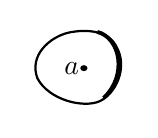
\begin{tikzpicture}[x=1cm,y=1cm]
\draw[line width=.8pt] (.03,.05) .. controls (-.08,.34) and (.18,.57) .. (.42,.63) .. controls (.65,.68) and (.94,.66) .. (1.04,.44) .. controls (1.18,.18) and (1.02,-.15) .. (.82,-.24) .. controls (.62,-.33) and (.18,-.23) .. (.03,.05) -- cycle;
\draw[line width=1.4pt] (.79,.64) .. controls (1.08,.57) and (1.18,.09) .. (.87,-.20);
\fill (.62,.18) ellipse (.046 and .038);
\node[left,inner sep=.7pt] at (.59,.18) {$a$};
\end{tikzpicture}}
(disque avec pt marqué) une figure de ce type, correspondant à $(B,\partial B)$, n'est pas \unsure{connue} par la seule connaissance de la partie (contractile etc) $\unsure{a|\bullet}$ de $B\setminus\partial B$ correspondant au ``centre'' du disque, mais il faut de plus se donner une ``structure de \unsure{reliement}'' de $a$ au bord\,\unsure{.....}.

Ceci étant, il est \inserted{sans doute} illusoire d'espérer que
\[
\begin{aligned}
&\deleted{\unsure{\mathcal F}\,\unsure{\mathrm{Mul}}\,\mathrm{mulomb}(F^{\unsure{\prime}})}\\
&\mathrm{mulomb}(F)\leq\mathrm{mulomb}(F')\Longrightarrow F\leq F'\\
&\mathrm{mulomb}(F)\ll\unsure{\mathrm{mulom}|\mathrm{mulomb}}(F')\Longrightarrow F\ll F',
\end{aligned}
\]
